\documentclass[11pt,a4paper]{article}
\usepackage[margin=1in]{geometry}
\usepackage{graphicx}
\usepackage{caption}
\usepackage{subcaption}
\usepackage{hyperref}
\usepackage{amsmath,amssymb}
\usepackage{booktabs}
\usepackage{algorithm}
\usepackage{algorithmic}
\usepackage{parskip}

\title{Exploring Classifier-Free Guidance in Diffusion Models}
\author{Dhruman Gupta, Rushil Gupta \\ Introduction to Machine Learning Final Project}
\date{\today}

\begin{document}
\maketitle

\begin{abstract}
We present an expository study of classifier-free guidance (CFG) in diffusion-based image generation. Leveraging a custom UNet trained on MS COCO captions with a frozen VAE and CLIP text encoder from Stable diffusion v1.4\cite{rombach2022stablediffusion}, we explore the qualitative effects of varying CFG weights on sample fidelity and diversity. Results showcase both successful generations on seen prompts and failure modes on novel objects.
\end{abstract}

\section{Introduction and Background}

Generative modeling has witnessed a renaissance with the advent of diffusion-based methods, which achieve remarkable fidelity by simulating a gradual denoising process. In this section, we first review the fundamentals of diffusion models, then discuss how conditioning can steer generation and introduce classifier guidance, and finally describe the more flexible classifier‐free guidance approach that forms the core of our project.

\subsection{Diffusion Models}

Diffusion models \cite{ho2020denoising} formulate generation as the reversal of a known, fixed noising process. The underlying idea is to "add noise" to the data distribution $p_{\mathrm{data}}(x)$, and then learn to reverse this process. By adding small amounts of noise, it becomes easier to learn the reverse process.\\

Consider a data distribution over images $x_0\sim p_{\mathrm{data}}(x)$, and define a forward Markov chain that progressively adds Gaussian noise:
\begin{equation}\label{eq:forward}
q(x_t \mid x_{t-1}) = \mathcal{N}\!\bigl(x_t;\,\sqrt{1-\beta_t}\,x_{t-1},\,\beta_t I\bigr),\quad t=1,\dots,T,
\end{equation}
where $\{\beta_t\}$ is a small, increasing variance schedule.  After $T$ steps, $x_T$ is essentially isotropic Gaussian noise. To generate new samples, we learn a parameterized reverse process
\begin{equation}\label{eq:reverse}
p_\theta(x_{t-1}\mid x_t) 
= \mathcal{N}\!\Bigl(x_{t-1};\,\mu_\theta(x_t,t),\,\sigma_t^2 I\Bigr),
\end{equation}
with mean
\[
\mu_\theta(x_t,t)
=\frac{1}{\sqrt{\alpha_t}}\Bigl(x_t-\frac{\beta_t}{\sqrt{1-\bar\alpha_t}}\;\epsilon_\theta(x_t,t)\Bigr),
\]
where $\alpha_t = 1-\beta_t$ and $\bar\alpha_t = \prod_{s=1}^t \alpha_s$.  The network $\epsilon_\theta(x_t,t)$ predicts the noise component at each step.  Training minimizes the denoising objective:
\begin{equation}\label{eq:loss}
\mathcal{L}(\theta)
=\mathbb{E}_{x_0,\epsilon,t}\Bigl[\bigl\|\epsilon-\epsilon_\theta(x_t,t)\bigr\|^2\Bigr],\quad
x_t=\sqrt{\bar\alpha_t}\,x_0+\sqrt{1-\bar\alpha_t}\,\epsilon,\;\epsilon\sim\mathcal{N}(0,I).
\end{equation}
In practice, this simple loss yields stable training and high-quality samples.

\begin{algorithm}[htb]
\caption{Unconditional DDPM Sampling}\label{alg:ddpm}
\begin{algorithmic}[1]
  \STATE \textbf{Input:} noise schedule $\{\beta_t\}_{t=1}^T$, learned model $\epsilon_\theta$
  \STATE $x_T \sim \mathcal{N}(0,I)$
  \FOR{$t=T,\dots,1$}
    \STATE $\hat\epsilon \leftarrow \epsilon_\theta(x_t,t)$
    \STATE $\mu \leftarrow \frac{1}{\sqrt{\alpha_t}}\Bigl(x_t - \tfrac{\beta_t}{\sqrt{1-\bar\alpha_t}}\hat\epsilon\Bigr)$
    \STATE Sample $x_{t-1}\sim \mathcal{N}(x_{t-1};\,\mu,\sigma_t^2 I)$
  \ENDFOR
  \STATE \textbf{return} $x_0$
\end{algorithmic}
\end{algorithm}

\subsection{Conditioning and Classifier Guidance}

While unconditional diffusion can produce diverse samples, many applications demand control over the output, such as generating an image of a specified class or matching a textual prompt $y$.  Ideally, one would sample from the conditional distribution $p(x_0\mid y)$.  Classifier guidance \cite{dhariwal2021diffusion} achieves this by leveraging an auxiliary classifier $p_\phi(y\!\mid\!x_t)$ trained on noisy inputs.\\


Since we want to sample from $p(x_0\mid y)$, we can use Bayes' rule and score decomposition to decompose the gradient:
\[
\nabla_{x_t}\log p(x_t\mid y)
=\nabla_{x_t}\log p(x_t)
+\nabla_{x_t}\log p(y\mid x_t),
\]
we adjust the denoising mean in the reverse step:
\begin{equation}\label{eq:clf_guidance}
\tilde{\mu}
=\mu_\theta(x_t,t)
+ s\,\sigma_t^2\,\nabla_{x_t}\log p_\phi(y\mid x_t),
\end{equation}
where $s$ is the guidance strength.  Intuitively, the classifier gradient pushes $x_t$ toward regions where the classifier predicts $y$.

\begin{algorithm}[htb]
\caption{Classifier‐Guided Sampling}\label{alg:clf_guidance}
\begin{algorithmic}[1]
  \STATE \textbf{Input:} schedule $\{\beta_t\}$, model $\epsilon_\theta$, classifier $p_\phi$, strength $s$
  \STATE $x_T \sim \mathcal{N}(0,I)$
  \FOR{$t=T,\dots,1$}
    \STATE $\hat\epsilon \leftarrow \epsilon_\theta(x_t,t)$
    \STATE $\mu \leftarrow \frac{1}{\sqrt{\alpha_t}}\bigl(x_t - \tfrac{\beta_t}{\sqrt{1-\bar\alpha_t}}\hat\epsilon\bigr)$
    \STATE $g \leftarrow \nabla_{x_t}\log p_\phi(y\!\mid\!x_t)$
    \STATE $\mu \leftarrow \mu + s\,\sigma_t^2\,g$
    \STATE Sample $x_{t-1}\sim\mathcal{N}(x_{t-1};\,\mu,\sigma_t^2 I)$
  \ENDFOR
  \STATE \textbf{return} $x_0$
\end{algorithmic}
\end{algorithm}

Although effective, classifier guidance requires training a separate classifier on every noise level and can incur significant compute overhead.  Moreover, classifier gradients may introduce artifacts if the classifier is imperfect.\\

Another flaw of the classifier guidance is that it only works for fixed classes, which the classifier is trained on. However, in many cases, we may want to generate samples from an evolving distribution of classes, which is not possible with classifier guidance.

\newpage

\subsection{Classifier‐Free Guidance}

Classifier‐free guidance (CFG) \cite{ho2022classifierfree} elegantly sidesteps the need for an external classifier by training the diffusion model itself to operate both with and without conditioning. The existing diffusion models can be thought of as conditional models that sample with condition $\varnothing$. Given training data with appropriate condition labels, we can train the model to sample from these conditions.\\

In classifier-free guidance, we train the model to sample from these conditions. However, for a more generalisable model, we also want it to sample unconditionally - this gives higher diversity. Thus, during training, the model is trained to sample from both $\varnothing$ and $c$:\\


During training, each sample's condition $c$ (e.g.\ text embedding) is randomly dropped with probability $p_\text{drop}$ (for example, $0.2$), so the model learns to predict
\[
\epsilon_\theta(x_t,t,c)\quad\text{and}\quad\epsilon_\theta(x_t,t,\varnothing)\,.
\]
At inference, one interpolates between these two predictions:
\begin{equation}\label{eq:cfg}
\epsilon_{\mathrm{CFG}}
=(1+w)\,\epsilon_\theta(x_t,t,c)\;-\;w\,\epsilon_\theta(x_t,t,\varnothing),
\end{equation}
where $w\ge0$ is the guidance weight.  Substituting $\epsilon_{\mathrm{CFG}}$ into the reverse mean (Eq.~\ref{eq:reverse}) yields a sample that balances fidelity to the condition against sample diversity.\\

Note: by adding the weight $w$, we actually end up samping from the following distribution:
\[
p_{\mathrm{CFG}}(x_0) = p(x_0\mid c)^{1+w}p(x_0)^{-w}.
\]

While this is not the same as sampling from $p(x_0\mid c)$, it often works better for generating images. Stable Diffusion uses $w=7.5$ as a general default. This value is often exposed as a parameter to the user in the pipeline.

\begin{algorithm}[htb]
\caption{Classifier‐Free Guidance Sampling}\label{alg:cfg}
\begin{algorithmic}[1]
  \STATE \textbf{Input:} schedule $\{\beta_t\}$, model $\epsilon_\theta$, weight $w$, condition $c$
  \STATE $x_T \sim \mathcal{N}(0,I)$
  \FOR{$t=T,\dots,1$}
    \STATE $\epsilon_c \leftarrow \epsilon_\theta(x_t,t,c)$
    \STATE $\epsilon_u \leftarrow \epsilon_\theta(x_t,t,\varnothing)$
    \STATE $\epsilon \leftarrow (1+w)\,\epsilon_c - w\,\epsilon_u$
    \STATE $\mu \leftarrow \frac{1}{\sqrt{\alpha_t}}\bigl(x_t - \tfrac{\beta_t}{\sqrt{1-\bar\alpha_t}}\epsilon\bigr)$
    \STATE Sample $x_{t-1}\sim\mathcal{N}(x_{t-1};\,\mu,\sigma_t^2 I)$
  \ENDFOR
  \STATE \textbf{return} $x_0$
\end{algorithmic}
\end{algorithm}

CFG offers several advantages: it requires no extra classifier, allows a single model to flexibly trade off between unconditional and conditional generation, and has been shown to deliver state‐of‐the‐art sample quality with minimal overhead.

\newpage

% --- UNet Explanation ---

% UNet: Architecture and Role in Diffusion Models

\subsection{UNet Architecture}
Finally, we need to understand the UNet architecture, which is the core of our model. The UNet architecture, originally introduced for biomedical image segmentation~\cite{ronneberger2015u}, has become a cornerstone for image-to-image tasks, including denoising and generative modeling. Its design enables the model to reverse a corruption process by progressively refining features at multiple spatial resolutions. The key idea is to combine high-resolution spatial information with deep, coarse features, thereby capturing both local and global context.

The UNet consists of three main components:
\begin{itemize}
    \item \textbf{Downsampling Path:} Stacks of convolutional layers (Conv$\rightarrow$ReLU$\rightarrow$Conv$\rightarrow$ReLU) progressively downsample the input, extracting increasingly abstract features.
    \item \textbf{Bottleneck:} The deepest layer, which captures the most abstract representation of the input. No pooling is used here—just convolutions.
    \item \textbf{Upsampling Path:} Upsampling layers (typically transposed convolutions) restore the spatial size, halving the number of channels at each step. Skip connections concatenate encoder feature maps to the decoder at each level, preserving fine-grained details lost during downsampling.
\end{itemize}

Each block also has a cross-attention layer, which allows the model to attend to the text prompt effectively. This architecture is particularly well-suited for diffusion models, as it allows the network to learn both global structure and local details necessary for high-fidelity image synthesis.

\begin{figure}[ht]
\centering
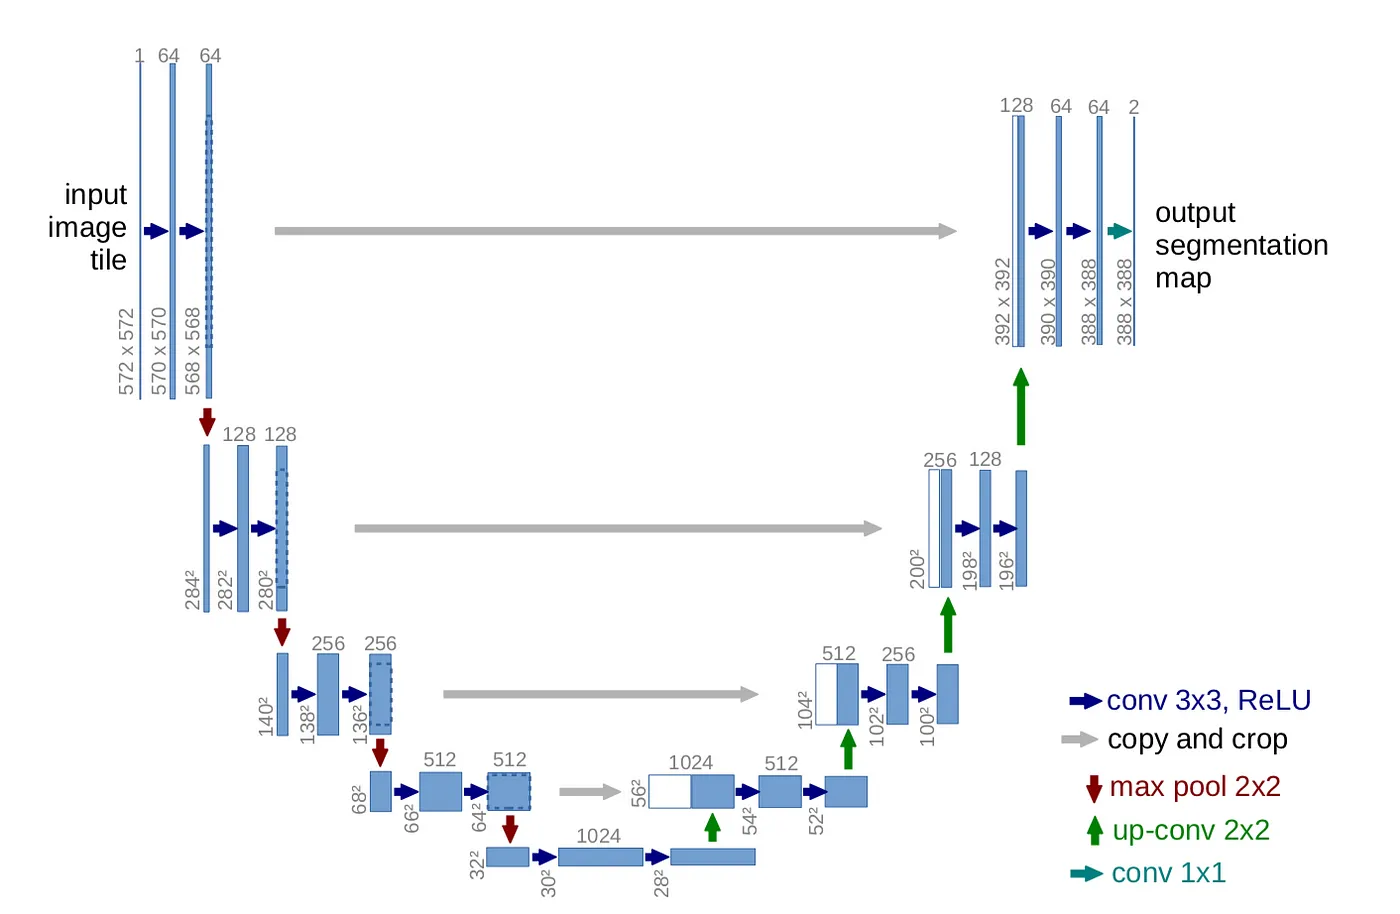
\includegraphics[width=0.69\textwidth]{figures/unet.png}
\caption{UNet architecture used for denoising in diffusion models.}
\end{figure}

% --- Dataset and Preprocessing ---

\section{Dataset and Preprocessing}

We use the MS COCO 2014 captions dataset, which contains $\sim$100,000 images annotated for object detection, segmentation, and captioning. The dataset comprises 80 categories, including common objects such as cars, bicycles, and animals, as well as more specific categories like umbrellas, handbags, and sports equipment. For our experiments, all images are resized to $128\times128$ pixels and center-cropped to ensure uniformity and compatibility with the model architecture.

During training, we employ a caption dropout strategy: for each sample, the text condition (caption) is randomly dropped with a fixed probability. This encourages the model to learn both conditional and unconditional generation, which is essential for classifier-free guidance.

% --- Model and Training ---

\section{Model and Training}

\paragraph{Architecture.} Our model leverages a frozen VAE and CLIP text encoder from Stable Diffusion v1.4\cite{rombach2022stablediffusion} to encode and decode images and text prompts, respectively. The core denoising network is a custom UNet, constructed with four downsampling and four upsampling blocks, each containing two layers. The cross-attention dimensions are set to match the CLIP encoder (768 channels).

\paragraph{Training Setup.} The diffusion process is set to 1,000 timesteps. We optimize the model using AdamW (learning rate $1\times10^{-4}$, weight decay $1\times10^{-2}$) and apply a CosineAnnealingLR schedule over 450 epochs. The batch size is 320, with gradient accumulation over 4 steps to accommodate hardware constraints.

\begin{algorithm}[htb]
\caption{Training Procedure for Classifier-Free Guided Diffusion}
\begin{algorithmic}[1]
  \STATE \textbf{Input:} Dataset $\mathcal{D} = \{(x_0, c)\}$, noise schedule $\{\beta_t\}_{t=1}^T$, dropout probability $P_{\mathrm{drop}}$
  \FOR{each minibatch}
    \STATE $(x_0, c) \sim \mathcal{D}$ \hfill // sample random data and condition
    \STATE $t \sim \mathrm{Uniform}(\{1, \ldots, T\})$ \hfill // sample timestep
    \STATE With probability $P_{\mathrm{drop}}$, $c \leftarrow \varnothing$ \hfill // drop condition
    \STATE $e_c = \mathrm{CLIP}(c)$ \hfill // encode $c$ using CLIP
    \STATE $z_0 = \mathrm{VAE}(x_0)$ \hfill // encode $x_0$ using VAE encoder
    \STATE $\epsilon \sim \mathcal{N}(0, I)$ \hfill // sample noise
    \STATE $z_t = \sqrt{\bar{\alpha}_t} z_0 + \sqrt{1 - \bar{\alpha}_t} \epsilon$ \hfill // add noise to $z_0$
    \STATE $\hat{\epsilon}_\theta = \epsilon_\theta(z_t, t, e_c)$ \hfill // predict noise
    \STATE Optimise for $\mathcal{L} = \|\epsilon - \hat{\epsilon}_\theta\|^2$
  \ENDFOR
\end{algorithmic}
\end{algorithm}

\begin{algorithm}[htb]
\caption{Sampling Procedure with Classifier-Free Guidance}
\begin{algorithmic}[1]
  \STATE \textbf{Input:} Condition $c$, guidance weight $w$, number of steps $T$
  \STATE Encode $c$ using CLIP: $e_c \leftarrow \mathrm{CLIP}(c)$
  \STATE $z_T \sim \mathcal{N}(0, I)$ \hfill // Sample initial latent
  \FOR{$t = T, \ldots, 1$}
    \STATE Predict $\epsilon_c = \epsilon_\theta(z_t, t, e_c)$
    \STATE Predict $\epsilon_u = \epsilon_\theta(z_t, t, \varnothing)$
    \STATE Compute guided noise: $\epsilon = (1 + w)\epsilon_c - w\epsilon_u$
    \STATE Compute mean: $\mu = \frac{1}{\sqrt{\alpha_t}} \left(z_t - \frac{\beta_t}{\sqrt{1 - \bar{\alpha}_t}} \epsilon \right)$
    \STATE Sample $z_{t-1} \sim \mathcal{N}(\mu, \sigma_t^2 I)$
  \ENDFOR
  \STATE Decode image: $\hat{x}_0 \leftarrow \mathrm{VAE\_dec}(z_0)$
  \STATE \textbf{return} $\hat{x}_0$
\end{algorithmic}
\end{algorithm}

\newpage

% --- Inference and Sampling ---

\section{Inference and Sampling}

For evaluation, we assemble systematically vary the classifier-free guidance weights $w \in \{1.0, 3.0, 5.0, 7.0\}$. To ensure reproducibility, both the random seed and the number of timesteps are fixed across all experiments. For each prompt and guidance weight, we generate a 2$\times$2 grid of samples, allowing for qualitative comparison of fidelity and diversity.

% --- Results ---

\section{Results}

We present qualitative results illustrating the effect of guidance weight on sample quality. Each figure shows nine samples for a given prompt and guidance weight.

\begin{figure}[!ht]
\centering
\begin{subfigure}[b]{0.24\textwidth}
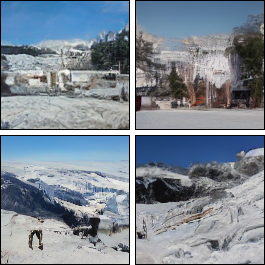
\includegraphics[width=\linewidth]{figures/a_beautiful_snowy_mountain_landscape_1.png}
\caption{$w=1.0$}
\end{subfigure}
\begin{subfigure}[b]{0.24\textwidth}
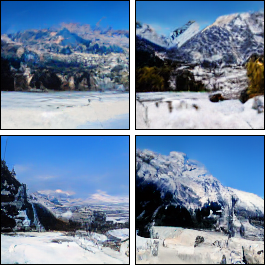
\includegraphics[width=\linewidth]{figures/a_beautiful_snowy_mountain_landscape_3.png}
\caption{$w=3.0$}
\end{subfigure}
\begin{subfigure}[b]{0.24\textwidth}
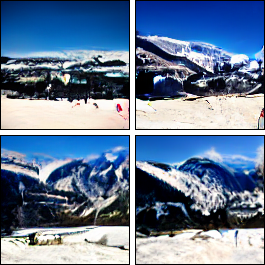
\includegraphics[width=\linewidth]{figures/a_beautiful_snowy_mountain_landscape_5.png}
\caption{$w=5.0$}
\end{subfigure}
\begin{subfigure}[b]{0.24\textwidth}
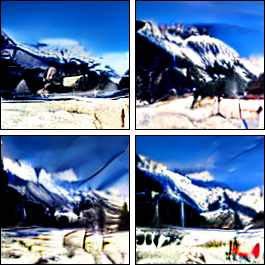
\includegraphics[width=\linewidth]{figures/a_beautiful_snowy_mountain_landscape_7.png}
\caption{$w=7.0$}
\end{subfigure}
\caption{Samples for the prompt ``a beautiful snowy mountain landscape'' at different guidance weights.}
\end{figure}

\begin{figure}[!ht]
\centering
\begin{subfigure}[b]{0.24\textwidth}
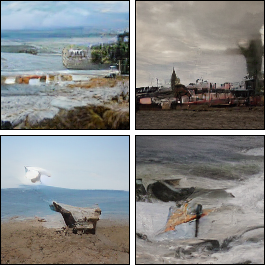
\includegraphics[width=\linewidth]{figures/a_beach_1.png}
\caption{$w=1.0$}
\end{subfigure}
\begin{subfigure}[b]{0.24\textwidth}
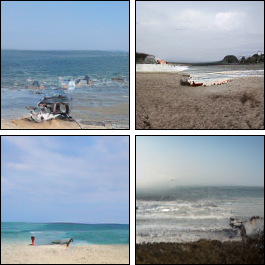
\includegraphics[width=\linewidth]{figures/a_beach_3.png}
\caption{$w=3.0$}
\end{subfigure}
\begin{subfigure}[b]{0.24\textwidth}
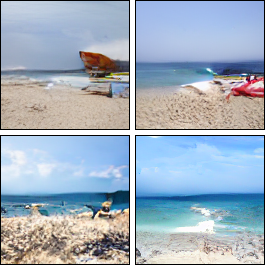
\includegraphics[width=\linewidth]{figures/a_beach_5.png}
\caption{$w=5.0$}
\end{subfigure}
\begin{subfigure}[b]{0.24\textwidth}
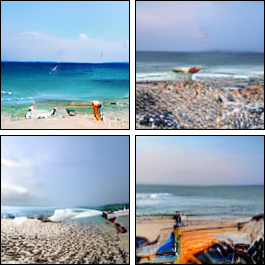
\includegraphics[width=\linewidth]{figures/a_beach_7.png}
\caption{$w=7.0$}
\end{subfigure}
\caption{Samples for the prompt ``a beach'' at different guidance weights.}
\end{figure}

\begin{figure}[!ht]
\centering
\begin{subfigure}[b]{0.24\textwidth}
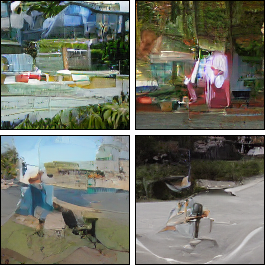
\includegraphics[width=\linewidth]{figures/A_tennis_court_1.png}
\caption{$w=1.0$}
\end{subfigure}
\begin{subfigure}[b]{0.24\textwidth}
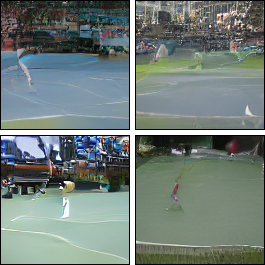
\includegraphics[width=\linewidth]{figures/A_tennis_court_3.png}
\caption{$w=3.0$}
\end{subfigure}
\begin{subfigure}[b]{0.24\textwidth}
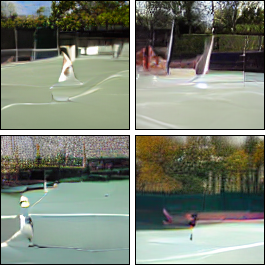
\includegraphics[width=\linewidth]{figures/A_tennis_court_5.png}
\caption{$w=5.0$}
\end{subfigure}
\begin{subfigure}[b]{0.24\textwidth}
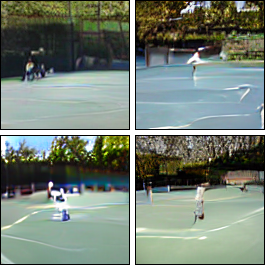
\includegraphics[width=\linewidth]{figures/A_tennis_court_7.png}
\caption{$w=7.0$}
\end{subfigure}
\caption{Samples for the prompt ``a tennis court'' at different guidance weights.}
\end{figure}

% --- Discussion ---

\section{Discussion}

Increasing the guidance weight $w$ enhances adherence to the prompt, resulting in samples that more closely match the intended description. However, this comes at the cost of reduced sample diversity, and at high values of $w$, the model can exhibit mode collapse. In our experiments, the limited dataset size and model capacity led to visible artifacts at high guidance weights. Failure cases on novel or uncommon objects further highlight the limitations of the MS COCO dataset, which lacks sufficient examples of rare items. The chosen UNet size represents a trade-off between computational feasibility and the ability to model complex scenes, and may underfit more intricate prompts.

% --- Future Work ---

\section{Future Work}

Future directions include expanding the training corpus with larger captioned datasets such as OpenImages or LAION to improve object diversity and generalization. Parameter-efficient fine-tuning methods (e.g., LoRA) could enable the use of larger backbone models within existing compute constraints. Additionally, exploring alternative noise schedules and reducing the number of diffusion timesteps may accelerate training and yield sharper images.

% --- Conclusion ---

\section{Conclusion}

We implemented classifier-free guidance in a custom diffusion model and systematically explored its qualitative impact. Our results demonstrate that classifier-free guidance provides a simple yet effective mechanism for balancing fidelity and diversity in generative image modeling. The findings underscore the importance of dataset scale and model capacity for achieving reliable and high-quality generative performance.

\bibliographystyle{plain}
\bibliography{refs}

\begin{thebibliography}{4}
    \bibitem{ho2020denoising}
    Ho, Jonathan, Ajay Jain, and Pieter Abbeel.
    \newblock Denoising Diffusion Probabilistic Models.
    \newblock In {\em Advances in Neural Information Processing Systems (NeurIPS)}, 2020.
    
    \bibitem{dhariwal2021diffusion}
    Dhariwal, Prafulla and Alex Nichol.
    \newblock Diffusion Models Beat GANs on Image Synthesis.
    \newblock In {\em Advances in Neural Information Processing Systems (NeurIPS)}, 2021.
    
    \bibitem{ho2022classifierfree}
    Ho, Jonathan and Tim Salimans.
    \newblock Classifier-Free Diffusion Guidance.
    \newblock In {\em Advances in Neural Information Processing Systems (NeurIPS)}, 2022.
    
    % Added U-Net citation
    \bibitem{ronneberger2015u}
    Ronneberger, Olaf, Philipp Fischer, and Thomas Brox.
    \newblock U-Net: Convolutional Networks for Biomedical Image Segmentation.
    \newblock arXiv preprint arXiv:1505.04597, 2015. \url{https://arxiv.org/abs/1505.04597}
    
    % Stable Diffusion citation
    \bibitem{rombach2022stablediffusion}
    Rombach, Robin, Andreas Blattmann, Dominik Lorenz, Patrick Esser, and Björn Ommer.
    \newblock High-Resolution Image Synthesis with Latent Diffusion Models.
    \newblock In \emph{Proceedings of the IEEE/CVF Conference on Computer Vision and Pattern Recognition (CVPR)}, 2022. \url{https://arxiv.org/abs/2112.10752}
    \end{thebibliography}
    
    \end{document}